\section{PID-results}

From an earlier project done by a summer-student at SINTEF, another controller has already been implemented. As a result, implementing SIMC or similar tuning methods is almost only interesting from the perspective of showing that it can be done. An easier approach is to make an automatic tuning algorithm that tries to improve on the parameters that have already been used.

\todo[inline]{Add the correct figures here and rewrite accordingly}
\noindent
If the simulator does not take too much time for each simulation, it is possible to automate parts of the tuning process and improve the controller by brute force  if some kind of measure of the quality can be found. Normally, a good measure for the quality of a controller will involve looking at overshoot, settling time and potential stationary deviation. In this case, the cost of the controller is instead deviation $e$ of the theoretical noise-free measurement $y_{\text{noise-free}}$ from the reference value.

\begin{align}
    \text{cost} = \left(\sum_{j=1}^m \sum_{i=1}^N \alpha_j \left(e_{T_i,j} \right)^2\right) + \sum_{j=1}^m \beta \max_{T_i} e_{T_i,j} + \sum \gamma_j \cdot |\sum_{i=1}^N e_{T_{i,j}}| \\
    \label{eq:simulation_cost}
\end{align}

Matlab has an implementation of the Nelder Mead algorithm in accordance to how it was described in \cite{Nelder_Mead_source}. This makes it possible to get good controllers by automatically tuning the parameters during the night. 

\noindent
The main drawback is that the algorithm still requires at least around 1000 iterations to find a really good solution. Additionally, the optimization does not take robustness or noise-rejection if it is not made into a part of the cost. 

An example of the progress of an automated tuning process can be seen in figure \ref{fig:optimization_progress}


\begin{figure}[!ht]
    \centering
    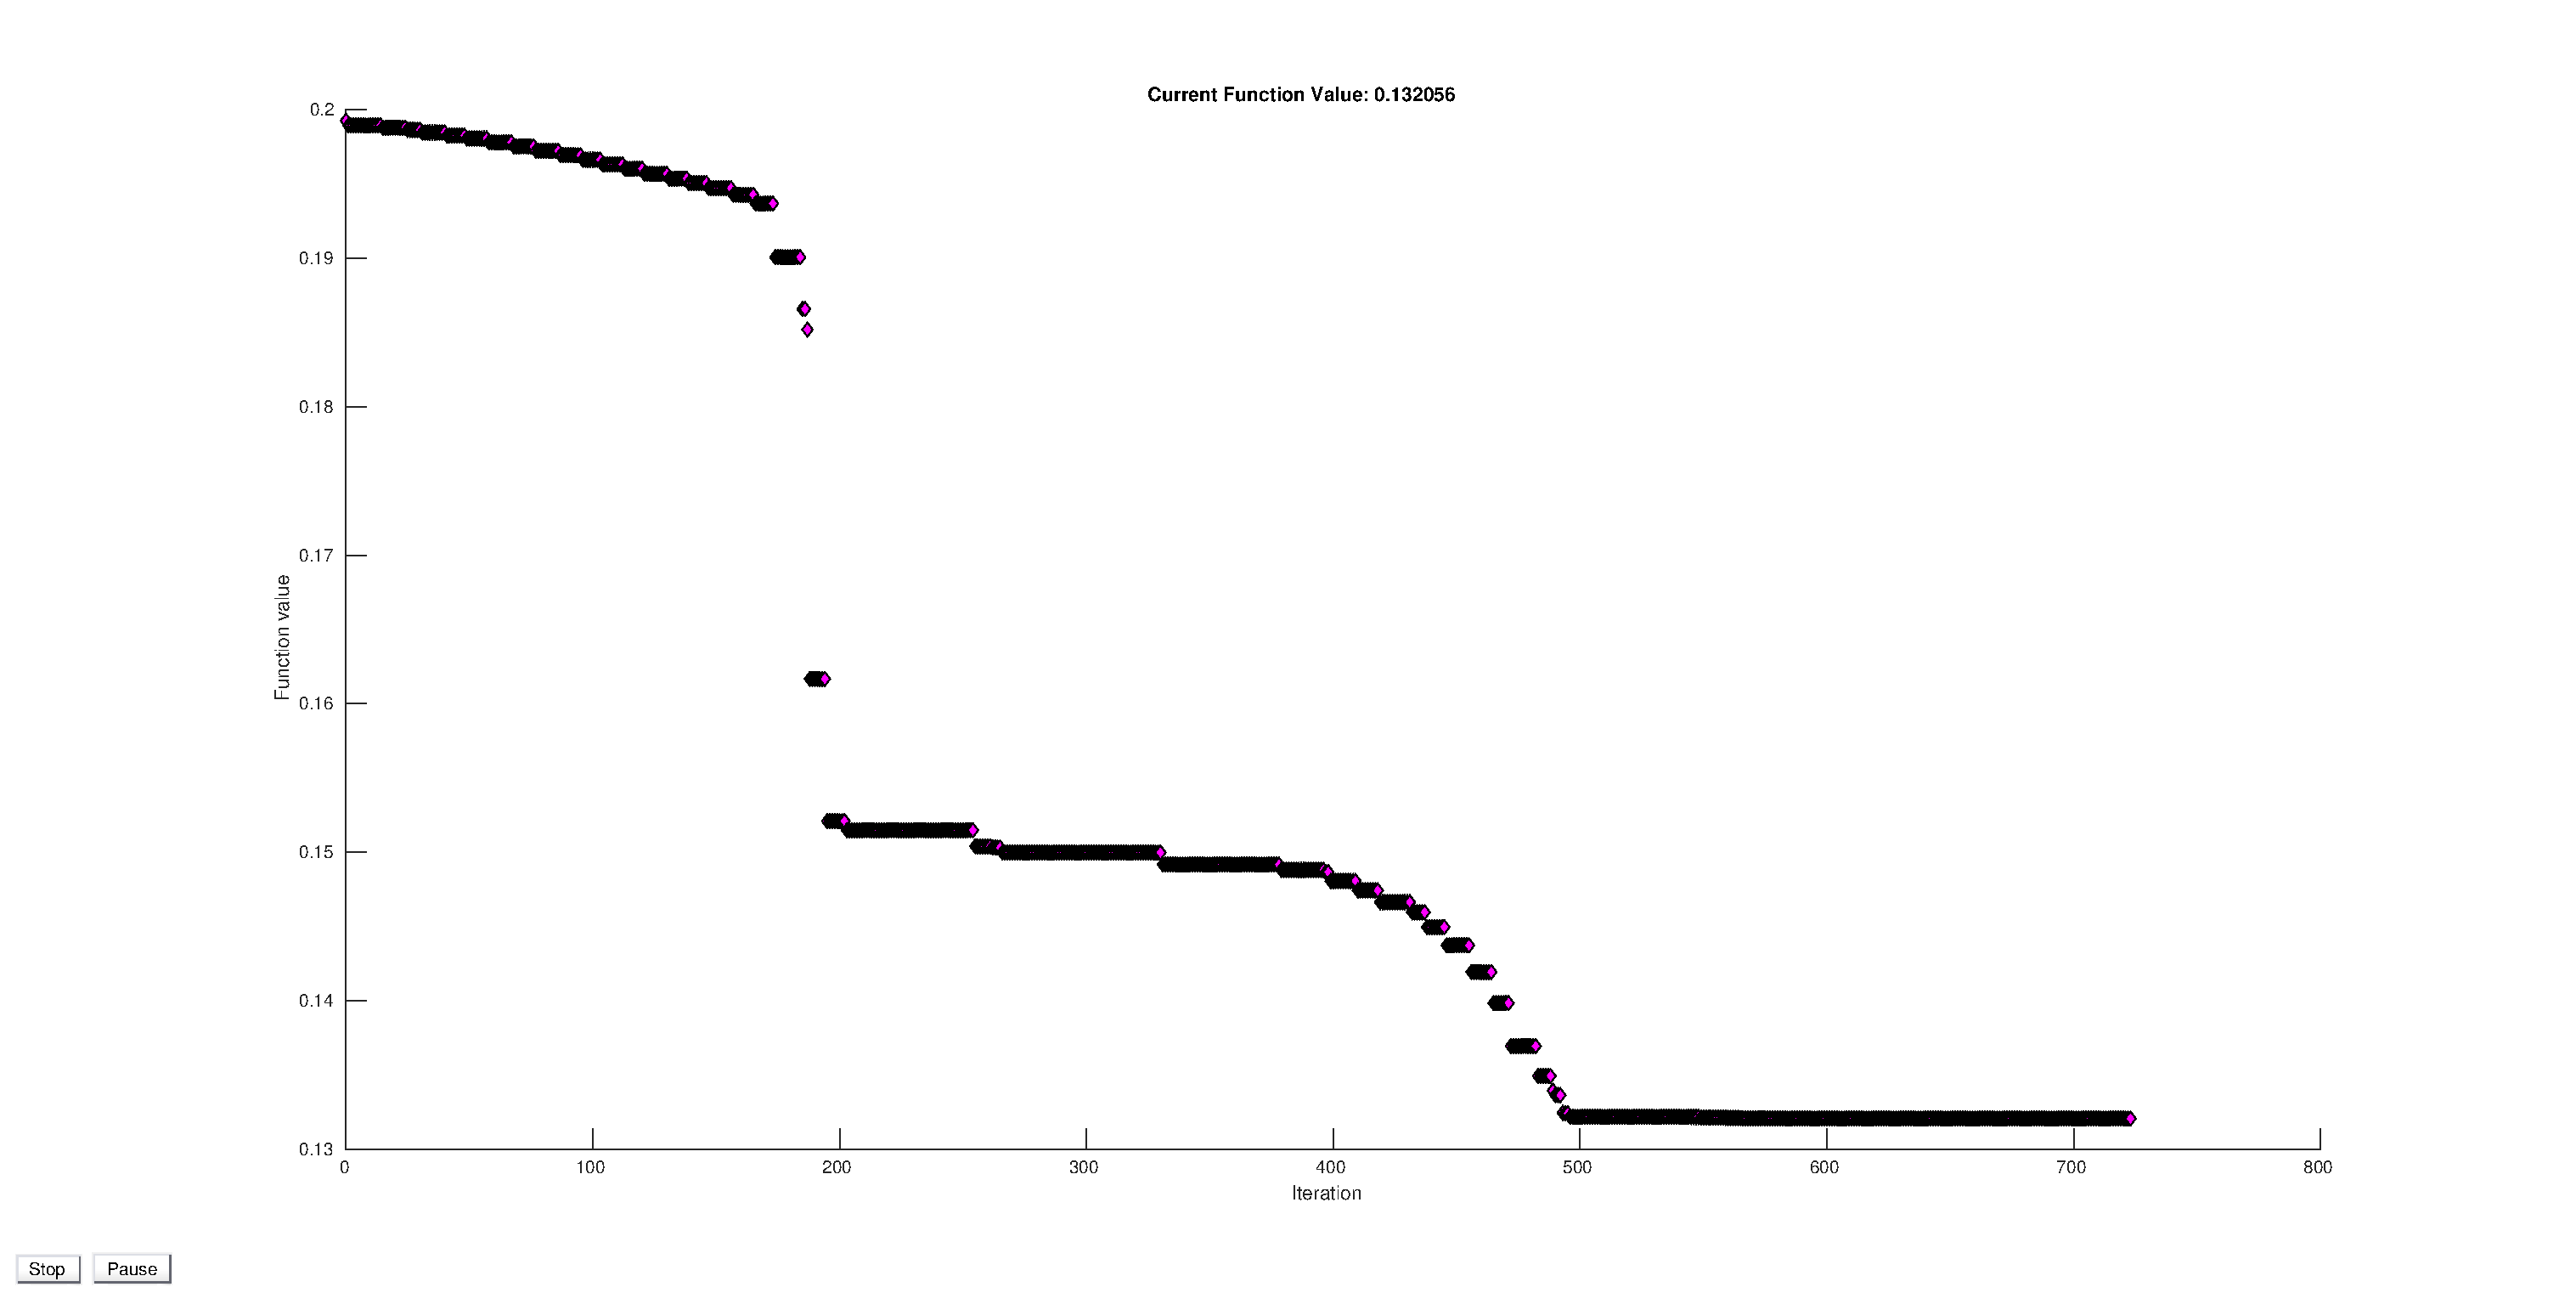
\includegraphics[width=\textwidth]{img/autotune_PID_progress.eps}
    \caption{Norm of $y(t) - y_{ref}(t)$ at each improved time-step of the Nelder-Mead optimization.}
    \label{fig:optimization_progress}
\end{figure}


\subsection{AB-controller}


\begin{figure}[!ht]
    \centering
    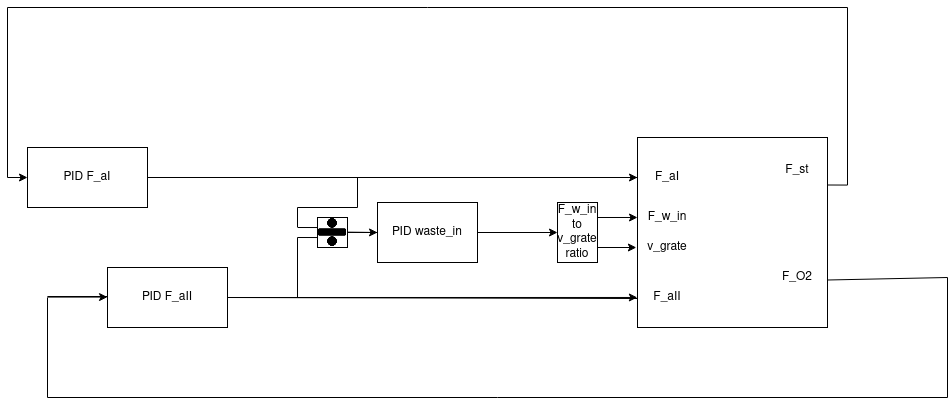
\includegraphics[width=\textwidth]{img/Fig_dump/AB_controller.png}
    \caption{A/B controller structure. Setpoints are assumed }
    \label{fig:AB_controller_structure}
\end{figure}


\noindent
Each output-variable is connected to one input-variable, with the secondary air being used to suppress any changes in the mass-flow of oxygen in the flue gas $F_{O2}$ and the primary air being used to suppress changes in the production of steam $F_{st}$. Using the primary air to control the steam production over long time-horizons is usually a bad idea since both a decent flow of primary and secondary air is needed for the gases to mix properly and for complete combustion to occur. As a result, the ratio between primary and secondary air $\frac{F_{aI}}{F_{aII}}$ is used as the final controlled variable in the plant. The controlled input-variable that is used to make this ratio follow the desired reference is a combination of grate-speed and the mass-flow of waste fed into the combustion chamber. A scaled difference could also have been used, but using a ratio may be desirable. Using too much secondary air is not too bad, beyond the loss of energy that comes from mixing the hot flue gas with ambient air. But using too little is potentially very bad since it might mean producing noxious gases.

\noindent


\begin{figure}[!ht]
    \centering
    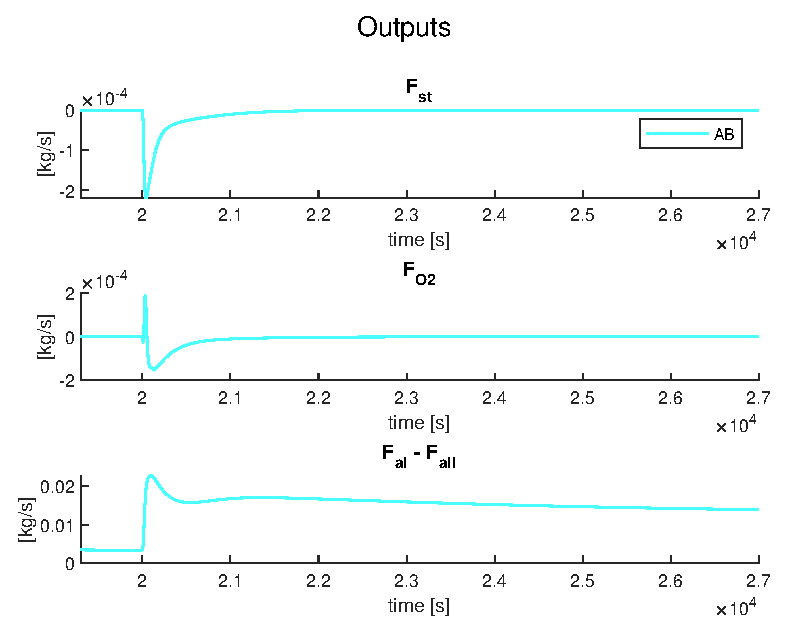
\includegraphics[width=\textwidth]{img/Fig_dump/outputs_ABStep_Q_all.eps}
    \caption{A/B controller disturbance step response}
    \label{fig:AB_outputs}
\end{figure}
\todo[inline]{@@@ Revert these figures to only use AB, instead of AB-cascade}

\begin{figure}[!ht]
    \centering
    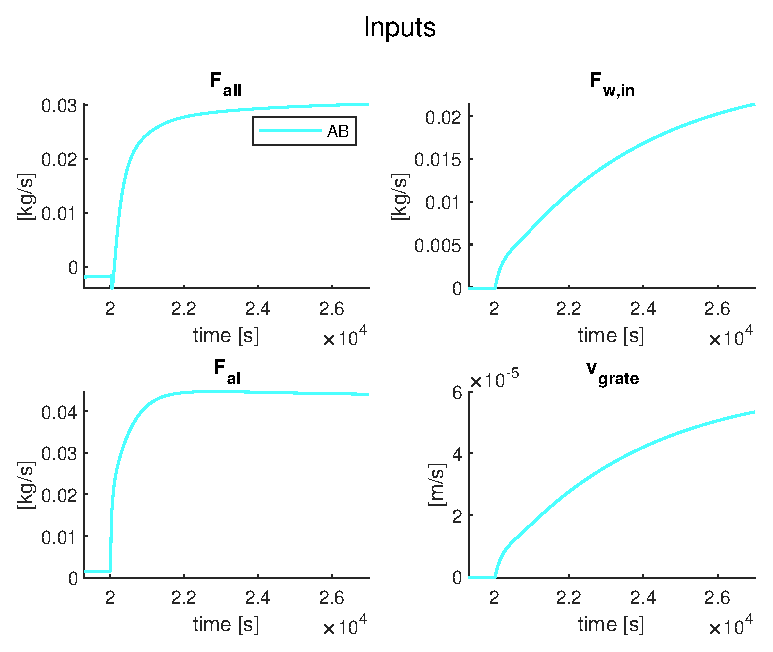
\includegraphics[width=\textwidth]{img/Fig_dump/inputs_ABStep_Q_all.eps}
    \caption{A/B controller disturbance step response}
    \label{fig:AB_inputs}
\end{figure}

Given a sudden step in process-disturbances, the change can be seen in \ref{fig:AB_outputs}. The change involves all three values for $Q_{\text{grate}}$ increasing by 50\%.  Regardless of the amount of measurement.-noise affecting the controller, low-pass filtering the signals still desirable as a safety-precaution. Due to the nature of the simulator having some pure feed-through terms, it is also necessary for completing a simulation. A basic continuous, linear, time-invariant low-pass filter with a time-constant of 0.1 was chosen.

\begin{align}
    \tau_{\text{low-pass}}= 0.1
\end{align}
The noise-spectrum may be very different, depending on the type of method that is used for measuring each variable. A common for of measurement-noise is the hum from the 50Hz AC-grid. The low-pass filter does serve the rejecting the noise from the AC-noise, but if the noise has a frequency-component around 1Hz that is too large, then the result will be far less pretty.

\begin{align}
    |\frac{1}{\left( 50 \cdot 2\pi \right) 0.1j+1}| \approx 0.0318
\end{align}

The response to a 50Hz noise-signal without any system disturbances is show in figure \ref{fig:AB_noise_response}


\begin{figure}[!ht]
    \centering
    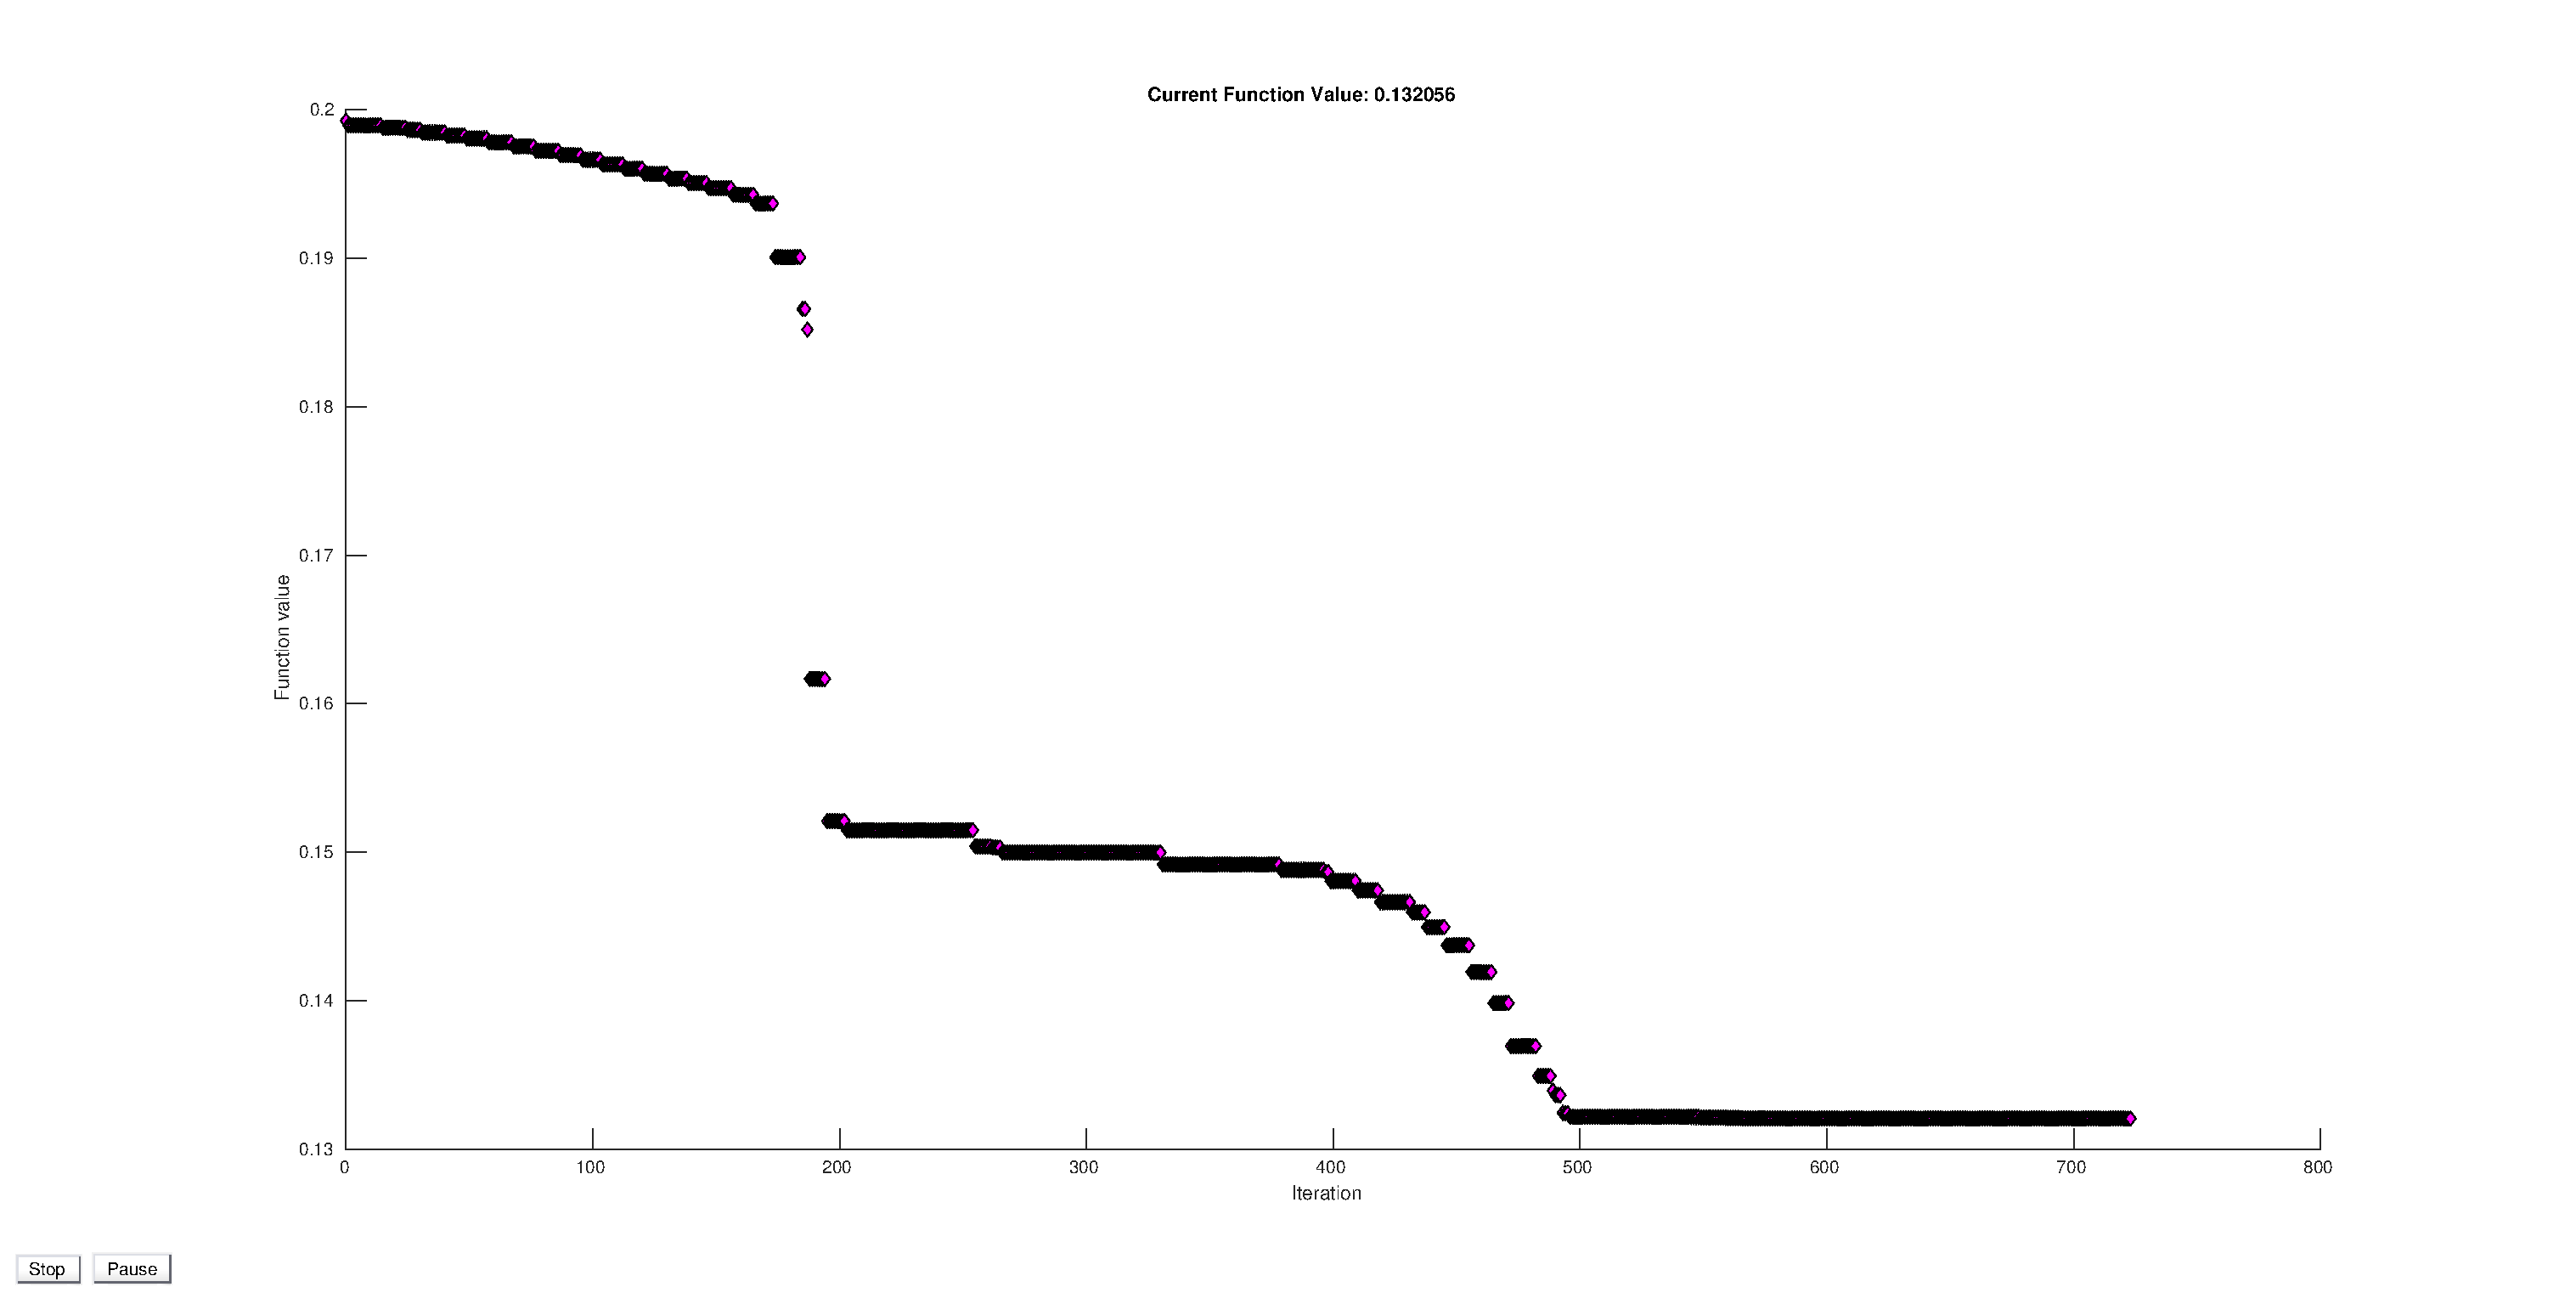
\includegraphics[width=\textwidth]{img/autotune_PID_progress.eps}
    \caption{A/B system noise-response@@@}
    \label{fig:AB_noise_response}
\end{figure}

The resulting response for the oxygen flow  $F_{O2}$ and the steam flow $F_{st}$ can be seen in figure \ref{fig:AB_outputs}.

\subsection{Cascaded A/B controller}
\cite{summer_student} also went on to investigate the possibilities of using a theoretical sensor measuring the heating value of the waste HHV when controlling the plant. The measure proposed there was an estimate

\begin{align}
    \hat{HHV} = \sum_j Cp_j F_{fg,j} \left( T_{fg} - T_{amb} \right)
\end{align}
which is the power delivered to the by a flow of flue-gas. The controller structure, as seen in figure \ref{fig:cascade_controller_structure} is the same as in \ref{fig:AB_controller_structure}, with the exception that the primary air is used to control $\hat{HHV}$, while the controller that tries to control the steam-production gives instead a reflue $\hat{HHV}$. The main advantage of using this controller should be that it can detect changes in the power delivered form combustion earlier, which allows for better control of the steam production. 

\begin{figure}[!ht]
    \centering
    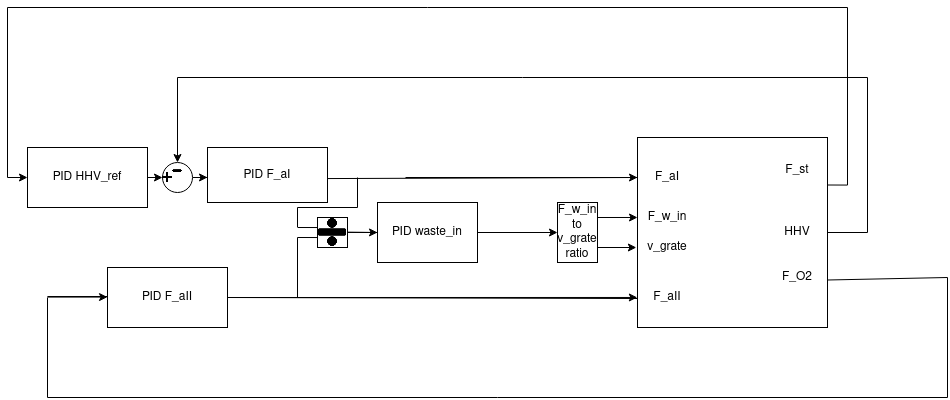
\includegraphics[width=\textwidth]{img/Fig_dump/cascaded_controller.png}
    \caption{Cascaded A/B controller structure}
    \label{fig:cascade_controller_structure}
\end{figure}


As can be seen, from figure \ref{fig:cascade_controller_structure}, both controllers have a rather similar response to changes in the waste quality when it comes to the oxygen concentration. The main advantage of using an estimate of the HHV-value when controlling the plant is the fact that the HHV-value changes before the steam-production, so the cascade controller can suppress the negative peak in the production of steam that happens for both the A/B-controller and the cascaded A/B-controller.

\begin{figure}[!ht]
    \centering
    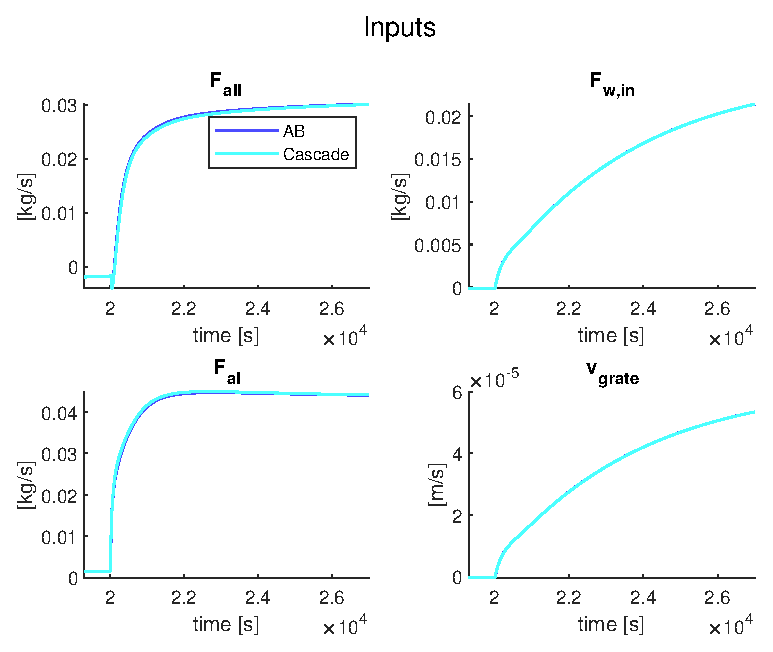
\includegraphics[width=\textwidth]{img/Fig_dump/inputs_ABCascadeStep_Q_all.eps}
    \caption{Cascaded A/B controller disturbance step response}
    \label{fig:cascade_controller_input_response}
\end{figure}




\begin{figure}[!ht]
    \centering
    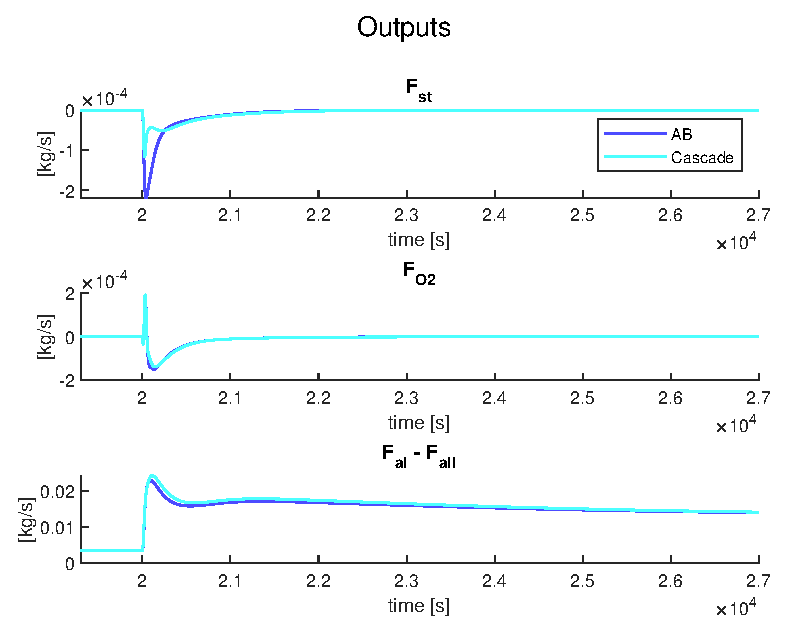
\includegraphics[width=\textwidth]{img/Fig_dump/outputs_ABCascadeStep_Q_all.eps}
    \caption{Cascaded A/B controller disturbance step response @@@ (Remove redundant AB) }
    \label{fig:cascade_controller_output_response}
\end{figure}


Figure \ref{fig:cascade_controller_output_response} has a noticeable in its response. It does not change the total amount of time needed to make the $F_{st}$ converge back to its reference, but the maximum amplitude of the error has decreased significantly. Additionally when looking at the changes in inputs needed to achieve this, figure \ref{fig:cascade_controller_input_response} shows that the inputs are almost identical, with the only difference being very slight differences in timing, with the cascaded controller being marginally more aggressive in its usage of primary air. 



